\title{Milestone 1}
\author{Singularity Software}
\date{\today}

\documentclass[12pt]{article}
\usepackage[a4paper]{geometry}
\usepackage{makeidx}
\usepackage{lscape}
\usepackage{amsmath}
\usepackage{graphicx}
\usepackage[final]{pdfpages}

\geometry{top=1.0in, bottom=1.0in, left=1.0in, right=1.0in} % Sets the margins

\setlength{\parindent}{0pt} % Fixes the paragraph spacing problem

\renewcommand*\arraystretch{1.5}

\begin{document}

\begin{center}
	\LARGE{Milestone 1} \\
	\Large{\textit{Singularity Software}} \\
	\vspace{.05in}
	\normalsize{\today} \\
\end{center}

\section*{Project Summary}
The Siftables Emulator is being developed by Singularity Software as part of the Junior Project sequence of classes at Rose-Hulman Institute of Technology. When projects were solicited for the sequence, clients Tim Ekl and Eric Stokes (both Rose-Hulman alumni) submitted a request for an emulator for Sifteo Cubes, a new platform intended for ``intelligent play." After Singularity was chosen for the project, we met with Mr. Ekl to determine the three primary features of the Emulator: a Workspace where 1-6 Cubes could mimic the manipulations possible with physical Cubes, an interface through which to program those virtual Cubes, and a set of example games designed to show off the first two features. Singularity's Emulator is intended to build on the foundation of Sifteo, Inc.'s existing emulator by creating a more fluid and natural user interface.
 \\\\
The clients' only implementation-specific specification was the ability to run the finished emulator on a Mac.

\section*{Weekly Meeting Time}
The team plans on meeting \textbf{each Sunday at 3 p.m.} to discuss that week's progress and what needs to be completed in the coming week. Other meeting times will be scheduled as needed.

\section*{Features}
\subsection*{Finished}

\begin{enumerate}
	\item{Visualizations of cube manipulations}
	\item{Zoom workspace}
	\item{Snap to grid}
	\item{Change number of cubes}
	\item{Recognization of cube neighboring}
	\item{Moving cubes}
	\item{Emulation utility methods (FillRect, Background)}
\end{enumerate}

\subsection*{Unfinished}
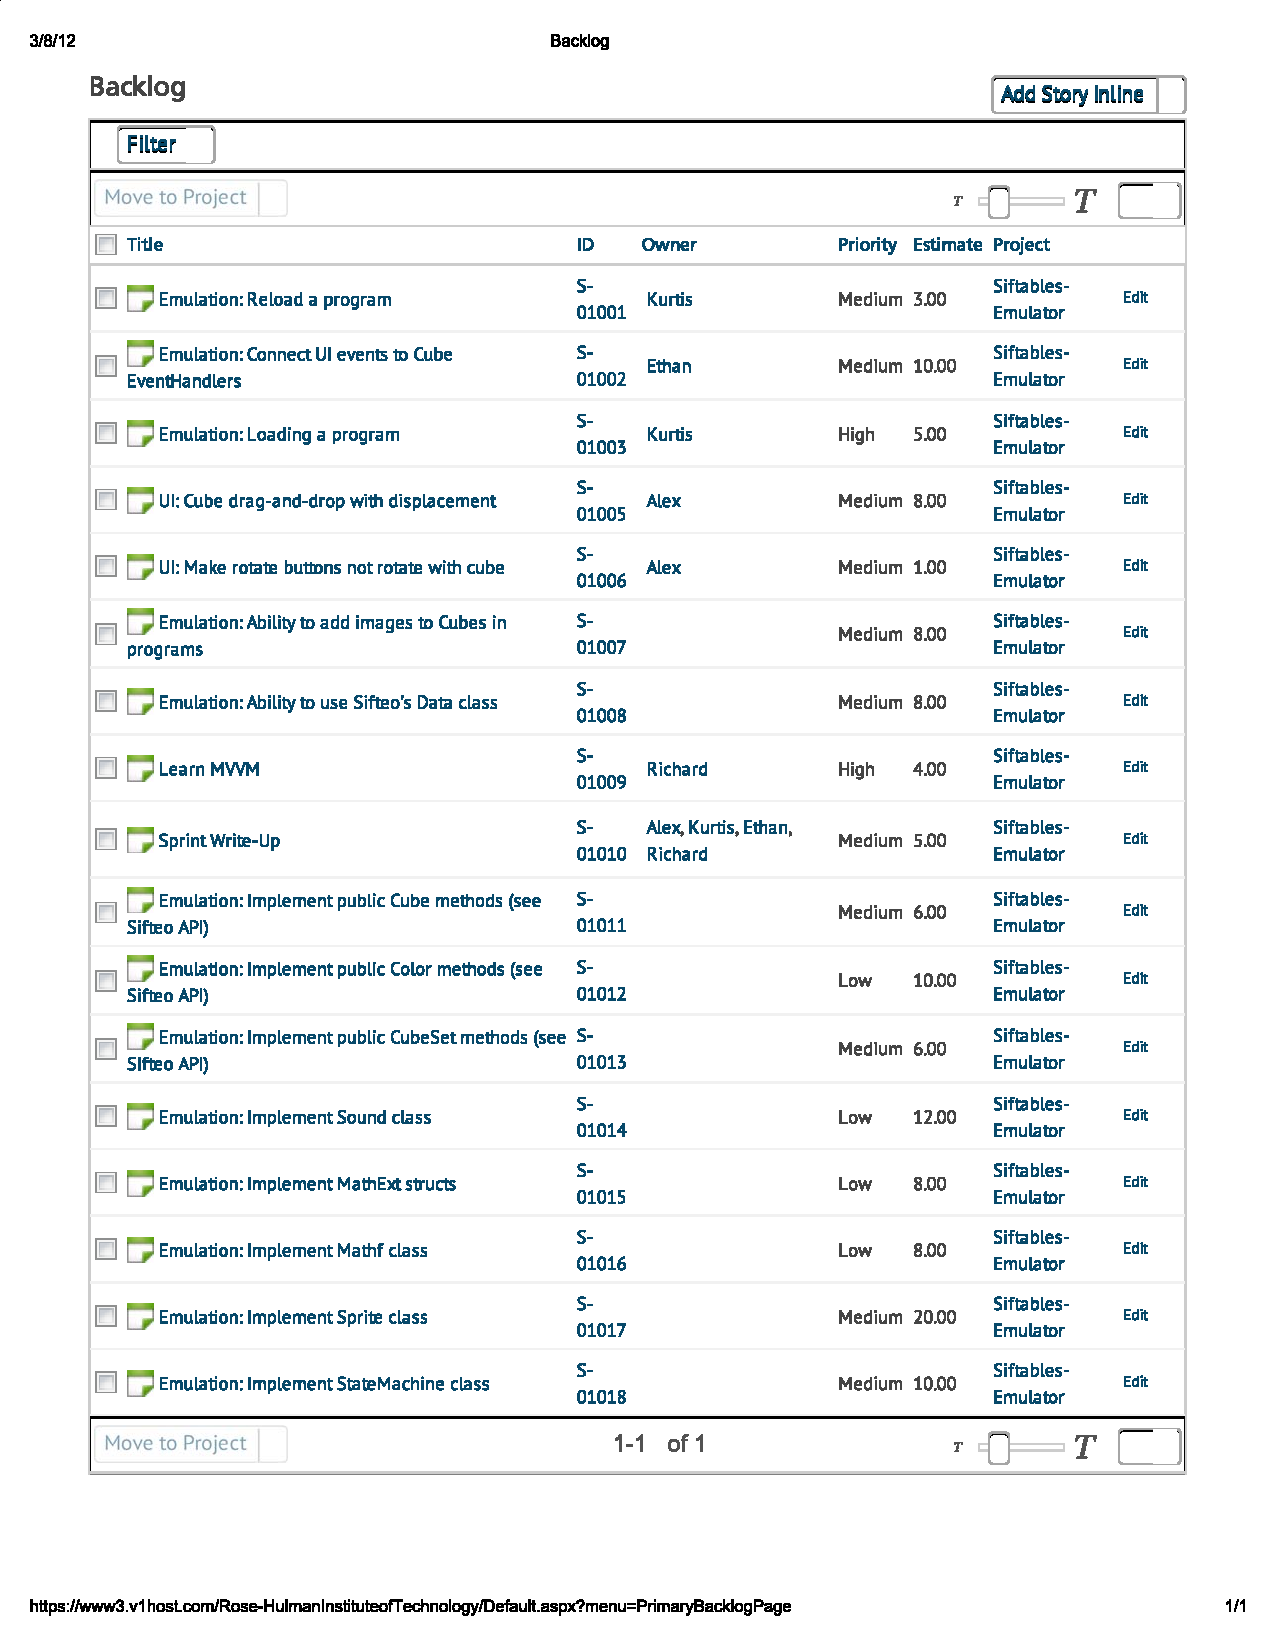
\includegraphics[scale=.75]{pdfs/MS1VersionOne/Backlog.pdf}

Priority is used as a substitute for an outright ordering of priority on tasks. In cases where a tie persists, tasks will be finished from top to bottom unless another ordering proves more prudent.

\section*{Two-Week Plan}
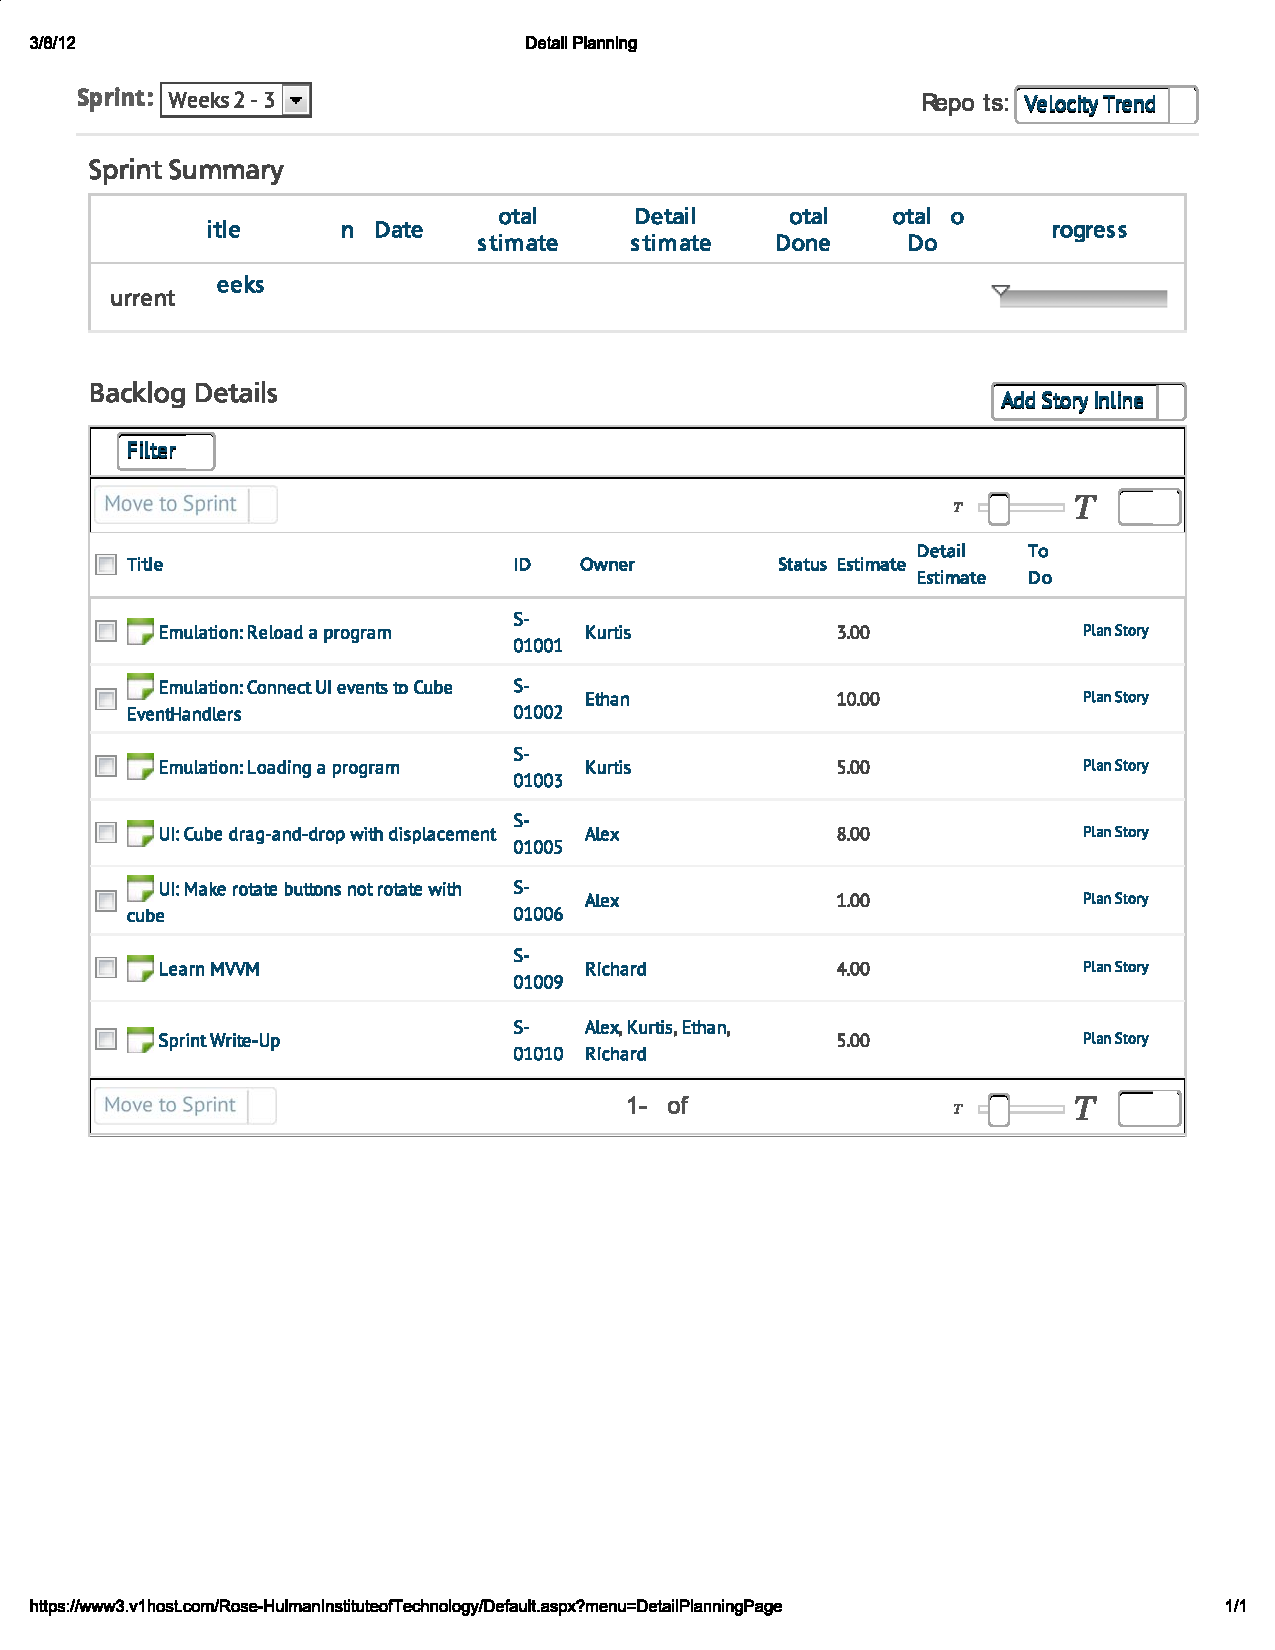
\includegraphics[scale=.75]{pdfs/MS1VersionOne/Sprint.pdf}
Due to the amount of design work completed previous to Richard joining the team, the team's goal is to have him familiar with the architecture and MVVM in general before embarking on tasks completely on his own.
        
\end{document}
